\section{ทฤษฎีที่เกี่ยวข้อง}

\subsection{การปกปิดข้อมูลในภาพและวิดีโอ}

การปกปิดข้อมูลภาพ (image obfuscation) เป็นกระบวนการลดรายละเอียดของบริเวณที่อาจเปิดเผยตัวตน โดยพยายามคงบริบทส่วนอื่นของภาพหรือวิดีโอให้สามารถนำไปใช้งานต่อได้ วิธีที่ใช้ในโครงงานประกอบด้วย Gaussian Blur, Pixelation และ Black Box วิธีแรกทำให้ค่าพิกเซลในบริเวณเป้าหมายเรียบขึ้นด้วยตัวกรองแบบเกาส์ วิธีที่สองลดความละเอียดเฉพาะบริเวณแล้วขยายกลับด้วยการประมาณค่าแบบเพื่อนบ้านใกล้ที่สุด ส่วนวิธีสุดท้ายแทนที่บริเวณเป้าหมายด้วยสีทึบทั้งหมด การเลือกระดับการปกปิดต้องคำนึงถึงทั้งความเป็นส่วนตัวและประโยชน์ใช้สอยของสื่อ เพราะการปกปิดที่อ่อนเกินไปอาจยังระบุตัวบุคคลได้ ขณะที่การปกปิดมากเกินไปอาจทำลายสาระสำคัญของภาพ

ระบบใช้ OpenCV สำหรับอ่าน เขียน และปรับแต่งเฟรมภาพหรือวิดีโอ\cite{bradski2000opencv} ก่อนใช้เอฟเฟกต์ ระบบจะตรวจสอบและจำกัดพิกัดกรอบให้อยู่ภายในขนาดเฟรมเสมอ เพื่อลดความผิดพลาดจากพิกัดที่ติดลบหรือเกินขอบภาพ

\subsection{Convolutional Neural Network(CNN)}

โครงข่ายประสาทเทียมแบบคอนโวลูชัน (Convolutional Neural Network: CNN) เป็นสถาปัตยกรรมที่ออกแบบให้เรียนรู้ลักษณะเชิงพื้นที่จากภาพโดยตรง ชั้นคอนโวลูชันใช้ตัวกรองขนาดเล็กเลื่อนไปบนภาพเพื่อสกัดลักษณะ เช่น ขอบ รูปร่าง และพื้นผิว ชั้นรวมค่า (pooling) ลดมิติของแผนที่ลักษณะและช่วยให้แบบจำลองทนต่อการเลื่อนตำแหน่งเล็กน้อย ส่วนชั้นเชื่อมต่อเต็มรูปแบบหรือชั้นทำนายจะรวมลักษณะที่เรียนรู้เพื่อจำแนกประเภทหรือประมาณตำแหน่งวัตถุ CNN จึงเป็นพื้นฐานสำคัญของทั้งตัวตรวจจับใบหน้าและแบบจำลองสร้างเวกเตอร์ลักษณะใบหน้าที่ใช้ในระบบ

\subsection{การตรวจจับใบหน้าหรือวัตถุด้วย YOLO}

YOLO หรือ You Only Look Once คือการตรวจจับวัตถุแบบเรียลไทม์ มีเป้าหมายในการระบุตำแหน่งและประเภทของวัตถุในภาพ ซึ่ง YOLO จะประมวลผลภาพในขั้นตอนเดียวและทำนายกรอบล้อมวัตถุพร้อมค่าความเชื่อมั่น\cite{redmon2016yolo} จึงเหมาะกับการประมวลผลเฟรมวิดีโอที่ต้องคำนึงถึงเวลา

ความโดดเด่นของ YOLO คือสามารถตรวจจับแม้กระทั่งวัตถุที่ซ้อนทับกันโดยมีโครงสร้างที่ค่อนข้างซับซ้อนของ grid ในแต่ละชั้นที่เล็กลงเรื่อยๆในแต่ละ layers

\subsection{วิธีตรวจจับใบหน้าแบบ Haar Cascade}

Haar Cascade เป็นวิธีตรวจจับวัตถุแบบดั้งเดิมที่ประเมินความแตกต่างของความเข้มระหว่างบริเวณสว่างและมืดด้วยคุณลักษณะคล้าย Haar การคำนวณผลรวมพิกเซลสามารถเร่งได้ด้วย integral image จากนั้น AdaBoost จะคัดเลือกคุณลักษณะที่จำแนกตัวอย่างบวกและลบได้ดี และจัดตัวจำแนกเป็นลำดับขั้น (cascade) เพื่อปฏิเสธบริเวณที่ไม่ใช่ใบหน้าอย่างรวดเร็ว\cite{viola2001}

วิธีนี้ใช้ทรัพยากรน้อยและทำงานแบบเวลาจริงได้ แต่ความแม่นยำอาจลดลงเมื่อใบหน้าเอียง แสงเปลี่ยนมาก หรือมีสิ่งบดบัง จึงนำมาอธิบายเพื่อแสดงพัฒนาการของงานตรวจจับใบหน้าและใช้เป็นแนวทางเปรียบเทียบกับแบบจำลองเชิงลึกในระบบปัจจุบัน


% ==================================================
% TODO IMAGE: ใส่ภาพประกอบทฤษฎีชนิดของคุณลักษณะ Haar
% Caption: ตัวอย่างคุณลักษณะ Haar แบบขอบ แบบเส้น และแบบสี่สี่เหลี่ยม
% หมายเหตุ: ตรวจสอบแหล่งที่มาของภาพและสิทธิ์การใช้งานก่อนนำมาใส่
% ==================================================
\begin{figure}[H]
\centering
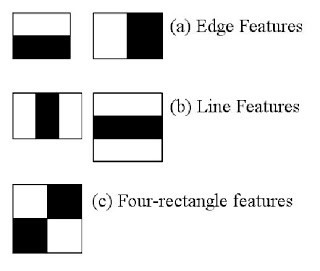
\includegraphics[width=0.8\textwidth]{images-progress/Haar feature.jpg}
\caption{ตัวอย่างคุณลักษณะ Haar แบบขอบ แบบเส้น และแบบสี่สี่เหลี่ยมที่ใช้ในตัวจำแนกแบบ Cascade}
\label{fig:haar-features}
\figuresource{OpenCV (ม.ป.ป.) \cite{opencv_haar_features}}
\figuredescription{fig:haar-features}{พื้นที่สีขาวและสีดำแทนบริเวณที่นำผลรวมค่าความเข้มของพิกเซลมาเปรียบเทียบ ภาพแสดงคุณลักษณะสามกลุ่ม ได้แก่ คุณลักษณะแบบขอบ (Edge Features) แบบเส้น (Line Features) และแบบสี่สี่เหลี่ยม (Four-rectangle Features) ซึ่งใช้ตรวจหารูปแบบความสว่างและความมืดที่สัมพันธ์กับส่วนประกอบของใบหน้า}
\end{figure}

\subsection{Support Vector Machine(SVM)}

Support Vector Machine: SVM เป็นวิธีการเรียนรู้แบบมีผู้สอนที่สร้างเส้นหรือระนาบแบ่งคลาส โดยกำหนดให้ระยะขอบระหว่างคลาสกว้างที่สุด ตัวอย่างที่อยู่ใกล้ระนาบแบ่งเรียกว่า support vectors และมีอิทธิพลต่อขอบเขตการตัดสินใจมากที่สุด สำหรับข้อมูลที่ไม่สามารถแบ่งเชิงเส้นได้ สามารถใช้ฟังก์ชันเคอร์เนลเพื่อแทนความสัมพันธ์ของข้อมูลในปริภูมิที่มีมิติสูงขึ้น

ในงานรู้จำใบหน้า SVM มักรับเวกเตอร์ลักษณะที่ผ่านการสกัดและลดมิติมาแล้วเพื่อจำแนกบุคคล อย่างไรก็ตาม ระบบปัจจุบันใช้การเปรียบเทียบเวกเตอร์ ArcFace ด้วย cosine similarity จึงกล่าวถึง SVM ในฐานะวิธีจำแนกทางเลือก ไม่ใช่ส่วนประกอบที่ใช้งานจริงในระบบ

\subsection{การรู้จำใบหน้าและการแทนลักษณะ}

การรู้จำใบหน้ามีเป้าหมายในการตรวจสอบหรือระบุอัตลักษณ์จากลักษณะของใบหน้า กระบวนการทั่วไปประกอบด้วยการปรับแนวใบหน้า การสกัดลักษณะ การสร้างตัวแทนเชิงตัวเลข และการเปรียบเทียบความคล้าย ระบบรู้จำใบหน้าต้องคำนึงถึงความเสี่ยงจากข้อมูลฝึก การรั่วไหลของตัวแทนใบหน้า และการนำผลไปใช้เกินวัตถุประสงค์\cite{sun2025}

ด้วยเหตุนี้ โครงงานจึงใช้ผลการรู้จำเพื่อจัดกลุ่มบุคคลภายในสื่อที่กำลังประมวลผลและให้ผู้ใช้ควบคุมการปกปิด โดยไม่เปิดเผยชื่อหรือข้อมูลอัตลักษณ์จริงของบุคคลที่ตรวจพบ

\subsubsection{Principal Component Analysis และ Eigenfaces}

Principal Component Analysis (PCA) ลดมิติข้อมูลโดยหาทิศทางที่มีความแปรปรวนสูง เมื่อประยุกต์กับใบหน้า ภาพแต่ละภาพถูกแปลงเป็นเวกเตอร์ $x_i$ และคำนวณใบหน้าเฉลี่ย
\begin{equation}
\psi=\frac{1}{m}\sum_{i=1}^{m}x_i.
\end{equation}
จากนั้นหาความแตกต่าง $a_i=x_i-\psi$ และสร้างเมทริกซ์ $A=[a_1,a_2,\ldots,a_m]$ เวกเตอร์ลักษณะเฉพาะที่สำคัญของเมทริกซ์ความแปรปรวนร่วมเป็นฐานของใบหน้าไอเกน (eigenfaces) ภาพใบหน้าสามารถประมาณในปริภูมิลดมิติได้เป็น
\begin{equation}
x_i-\psi \approx \sum_{j=1}^{K}w_j u_j,
\end{equation}
เมื่อ $u_j$ คือใบหน้าไอเกนและ $w_j$ คือน้ำหนักของภาพ วิธีนี้ลดภาระการคำนวณและใช้เปรียบเทียบใบหน้าได้ แต่ไวต่อแสง ท่าทาง และสิ่งบดบังมากกว่าวิธีเชิงลึกสมัยใหม่

% ==================================================
% TODO IMAGE: ใส่ภาพประกอบทฤษฎี Eigenfaces จากกระบวนการ PCA
% Caption: ตัวอย่างใบหน้าไอเกนจากกระบวนการ PCA
% แหล่งภาพที่ระบุใน Word: GeeksforGeeks, Face Recognition Using Eigenfaces
% ==================================================
\begin{figure}[H]
\centering
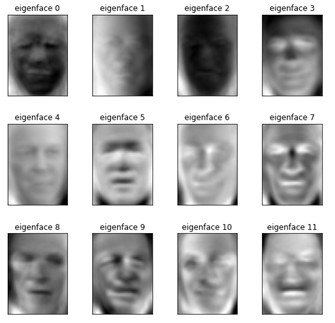
\includegraphics[width=0.8\textwidth]{images-progress/Face Recognition.jpg}
\caption{ตัวอย่างใบหน้าไอเกนจากกระบวนการ PCA}
\label{fig:pca-eigenfaces}
\figuresource{GeeksforGeeks (2021) \cite{geeksforgeeks2021eigenfaces}}
\figuredescription{fig:pca-eigenfaces}{ภาพแสดงใบหน้าไอเกนจำนวน 12 องค์ประกอบ โดยแต่ละองค์ประกอบแทนทิศทางความแปรปรวนหลักของข้อมูลใบหน้า เมื่อนำองค์ประกอบเหล่านี้มารวมกันด้วยค่าน้ำหนักที่เหมาะสมจะสามารถประมาณภาพใบหน้าในปริภูมิที่มีมิติลดลงได้}
\end{figure}

\subsubsection{Linear Discriminant Analysis และ Fisherfaces}

Linear Discriminant Analysis (LDA) เลือกทิศทางฉายข้อมูลที่เพิ่มความแตกต่างระหว่างคลาสและลดการกระจายภายในคลาส เมื่อนำมาใช้กับใบหน้า ตัวแทนที่ได้มักเรียกว่า Fisherfaces วิธีนี้ใช้ข้อมูลป้ายกำกับของบุคคลและอาจทนต่อความแปรผันภายในบุคคลได้ดีกว่า PCA ในบางกรณี อย่างไรก็ตาม ประสิทธิภาพยังขึ้นกับจำนวนและความหลากหลายของตัวอย่างฝึก

% ==================================================
% TODO IMAGE: ใส่ภาพประกอบทฤษฎี Fisherfaces จากกระบวนการ LDA
% Caption: ตัวอย่างใบหน้า Fisherfaces จากกระบวนการ LDA
% แหล่งภาพที่ระบุใน Word: BaseApp, Linear Discriminant Analysis
% ==================================================
\begin{figure}[H]
\centering
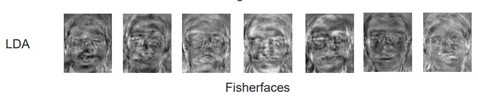
\includegraphics[width=0.8\textwidth]{images-progress/Fisherfaces.jpg}
\caption{ตัวอย่างใบหน้า Fisherfaces จากกระบวนการ LDA}
\label{fig:lda-fisherfaces}
\figuresource{Scholarpedia (ม.ป.ป.) \cite{scholarpedia_fisherfaces}}
\figuredescription{fig:lda-fisherfaces}{ภาพแสดงตัวแทน Fisherfaces ที่ได้จากการฉายข้อมูลด้วย LDA ซึ่งมุ่งเน้นลักษณะที่ช่วยเพิ่มความแตกต่างระหว่างกลุ่มบุคคลและลดความแปรปรวนของตัวอย่างภายในบุคคลเดียวกัน}
\end{figure}

\subsubsection{Elastic Bunch Graph Matching}

Elastic Bunch Graph Matching (EBGM) แทนใบหน้าเป็นกราฟของจุดสำคัญ เช่น ดวงตา จมูก และมุมปาก แต่ละจุดอธิบายด้วยผลตอบสนองของ Gabor wavelet และเชื่อมโยงกันด้วยความสัมพันธ์เชิงเรขาคณิต เมื่อเปรียบเทียบใบหน้า ระบบจะปรับกราฟให้สอดคล้องกับภาพใหม่แล้ววัดความคล้ายของลักษณะเฉพาะและตำแหน่งจุด วิธีนี้อธิบายโครงสร้างใบหน้าได้ชัดเจน แต่มีต้นทุนการกำหนดจุดและการจับคู่สูงกว่าแนวทางที่ใช้เวกเตอร์ลักษณะในระบบปัจจุบัน

% ==================================================
% TODO IMAGE: ใส่ภาพประกอบทฤษฎีการกำหนดจุดสำคัญบนใบหน้าด้วย EBGM
% Caption: การเปรียบเทียบจุดสำคัญที่กำหนดด้วยมือและตรวจจับอัตโนมัติด้วย Gabor-EBGM และ HOG-EBGM
% แหล่งภาพที่ระบุใน Word: ScienceDirect, Elastic Bunch Graph Matching
% ==================================================
\begin{figure}[H]
\centering
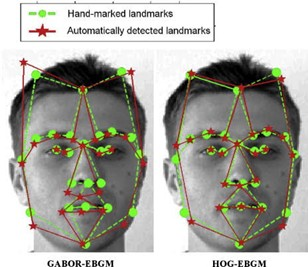
\includegraphics[width=0.8\textwidth]{images-progress/EBGM.jpg}
\caption{การเปรียบเทียบจุดสำคัญที่กำหนดด้วยมือและตรวจจับอัตโนมัติด้วย Gabor-EBGM และ HOG-EBGM}
\label{fig:ebgm-landmarks}
\figuresource{Albiol และคณะ (2008) \cite{albiol2008hogebgm}}
\figuredescription{fig:ebgm-landmarks}{วงกลมสีเขียวแสดงจุดสำคัญที่กำหนดด้วยมือ ส่วนสัญลักษณ์ดาวสีแดงแสดงจุดที่ตรวจจับโดยอัตโนมัติ ภาพด้านซ้ายเป็นผลของ Gabor-EBGM และภาพด้านขวาเป็นผลของ HOG-EBGM โดยเส้นเชื่อมระหว่างจุดแสดงโครงสร้างเชิงเรขาคณิตที่ใช้ประกอบการจับคู่ใบหน้า}
\end{figure}

\subsubsection{ArcFace และการจัดกลุ่มบุคคล}

ArcFace เป็นวิธีสร้างเวกเตอร์ลักษณะใบหน้าที่เพิ่ม angular margin ระหว่างคลาส เพื่อให้ตัวแทนของบุคคลต่างกันแยกออกจากกันได้ชัดเจนขึ้น\cite{deng2019arcface} การเปรียบเทียบเวกเตอร์สามารถใช้ cosine similarity เพื่อวัดความคล้ายระหว่างใบหน้า

ระบบปัจจุบันตัดภาพบริเวณใบหน้าพร้อมขยายขอบเขตบางส่วน แล้วสร้างเวกเตอร์ลักษณะด้วย InsightFace/ArcFace จากนั้นจึงปรับเวกเตอร์ให้มีขนาดหนึ่งและเปรียบเทียบกับกลุ่มบุคคลเดิม หากค่าความคล้ายผ่านเกณฑ์ที่กำหนด ระบบจะรวมใบหน้าเข้ากับกลุ่มเดิม มิฉะนั้นจะสร้างกลุ่มใหม่ กระบวนการนี้ทำให้ผู้ใช้เห็น Face Map เป็นรายการบุคคลแทนการเลือกกรอบใบหน้าทีละเฟรม

\subsection{การติดตามกรอบวัตถุ}

กรอบที่ตรวจพบระหว่างเฟรมถูกจับคู่ด้วยค่า Intersection over Union (IoU) และ Hungarian Algorithm หลักการดังกล่าวสอดคล้องกับการติดตามหลายวัตถุแบบออนไลน์ เช่น SORT\cite{bewley2016sort} ตัวติดตามในระบบเก็บอายุ จำนวนครั้งที่ตรวจพบ และความเร็วโดยประมาณของแต่ละกรอบ เพื่อลดการสูญหายของตำแหน่งในช่วงเวลาสั้น ๆ

สำหรับ Manual Control ระบบใช้ KCF เป็นตัวเลือกแรกและใช้ CSRT เมื่อ KCF ไม่พร้อม เพื่อให้กรอบที่ผู้ใช้วาดเคลื่อนตามวัตถุในวิดีโอ

\subsection{การตรวจจับข้อความและข้อมูลส่วนบุคคลจากข้อความ}

Optical Character Recognition (OCR) แปลงตัวอักษรในภาพเป็นข้อความดิจิทัล ส่วน Natural Language Processing (NLP) สามารถนำข้อความดังกล่าวไปจำแนกหรือระบุหน่วยข้อมูล เช่น ชื่อ หมายเลขโทรศัพท์ หรือข้อมูลส่วนบุคคลประเภทอื่น

แนวทางนี้มีประโยชน์ต่อการปกปิดข้อมูลที่ไม่ใช่ใบหน้า แต่ยังไม่ได้เชื่อมเข้ากับระบบต้นแบบปัจจุบัน จึงกำหนดไว้เป็นแนวทางพัฒนาต่อ โดยต้องประเมินทั้งความถูกต้องของ OCR และความครอบคลุมของตัวตรวจจับข้อมูลส่วนบุคคล

\subsection{สถาปัตยกรรมเว็บแอปพลิเคชัน}

ส่วนติดต่อผู้ใช้สร้างด้วย Next.js และ React ส่วน API และงานประมวลผลสร้างด้วย FastAPI ซึ่งรองรับการพัฒนา API ด้วยภาษา Python และการทำงานแบบ asynchronous\cite{fastapi} โดย Next.js ทำหน้าที่เป็นชั้น route handler ที่ส่งต่อคำขอจากเบราว์เซอร์ไปยัง FastAPI เพื่อลดการผูกส่วนหน้ากับตำแหน่งของส่วนหลังโดยตรง

ข้อมูลเมตาของวิดีโอและผลการตรวจจับจัดเก็บผ่าน SQLAlchemy ลงในฐานข้อมูล SQLite สำหรับระบบต้นแบบ ส่วนไฟล์ผลลัพธ์สามารถอัปโหลดไปยัง Cloudinary เมื่อมีการกำหนดข้อมูลรับรองที่จำเป็น

\section{งานวิจัยและงานที่เกี่ยวข้อง}

งานด้าน privacy-preserving video analytics ต้องแก้ปัญหาต่อเนื่องอย่างน้อยสามส่วน ได้แก่ การตรวจจับเป้าหมาย การติดตามเป้าหมายข้ามเฟรม และการปกปิดข้อมูลโดยยังคงประโยชน์ใช้สอยของสื่อไว้ PrivacyProber เสนอแนวทางประเมินและตรวจจับเทคนิคการเพิ่มความเป็นส่วนตัวเชิงซอฟต์ไบโอเมตริกซ์ ซึ่งสะท้อนว่าการประเมินความเป็นส่วนตัวไม่ควรพิจารณาเพียงว่ามีเอฟเฟกต์ปกปิดหรือไม่ แต่ต้องพิจารณาความสามารถในการดึงลักษณะระบุตัวตนหลังการปกปิดด้วย\cite{rot2022}

งานด้านป้ายทะเบียนแสดงให้เห็นว่าข้อมูลระบุตัวบุคคลในภาพไม่ได้จำกัดอยู่ที่ใบหน้า ทั้งงานสำรวจวิธีตรวจจับป้ายทะเบียน\cite{iiieta_anpr} ระบบจดจำป้ายทะเบียนที่ใช้ YOLOv8\cite{mdpi_anpr} และงานศึกษาการโจมตีเชิงปฏิปักษ์ต่อระบบอ่านป้ายทะเบียน\cite{vizcarra2024} ล้วนชี้ถึงความจำเป็นของการตรวจจับที่ทนต่อสภาพแวดล้อมหลากหลาย ขณะที่ชุดข้อมูลป้ายทะเบียนแบบนิรนาม\cite{anpr_dataset} เป็นตัวอย่างของการเตรียมข้อมูลที่ลดความเสี่ยงด้านความเป็นส่วนตัว

โครงงานนี้นำแนวคิดดังกล่าวมารวมเป็นเว็บแอปพลิเคชันที่ผู้ใช้ควบคุมผลการปกปิดได้เอง แตกต่างจากการเบลออัตโนมัติแบบตายตัว เพราะผู้ใช้สามารถยกเว้นบุคคลบางราย เลือกเอฟเฟกต์ และเพิ่มกรอบปกปิดให้วัตถุที่แบบจำลองยังไม่ครอบคลุม ตารางที่ \ref{tab:related-approach} สรุปความเชื่อมโยงระหว่างทฤษฎีกับส่วนที่นำไปใช้จริง

\begin{table}[H]
\centering
\caption{แนวคิดที่เกี่ยวข้องและการนำไปใช้ในระบบ}
\label{tab:related-approach}
\begin{tabular}{|p{0.28\textwidth}|p{0.30\textwidth}|p{0.27\textwidth}|}
\hline
\textbf{แนวคิด} & \textbf{บทบาท} & \textbf{การนำไปใช้} \\
\hline
YOLO & ตรวจหาตำแหน่งเป้าหมายในภาพ & ตรวจกรอบใบหน้าในแต่ละเฟรม \\
\hline
ArcFace Embedding & แยกความแตกต่างของบุคคล & จัดกลุ่มใบหน้าและสร้าง Face Map \\
\hline
IoU และ Hungarian Matching & จับคู่กรอบข้ามเฟรม & รักษากลุ่มบุคคลและตำแหน่งกรอบเมื่อวิดีโอเคลื่อนไหว \\
\hline
KCF/CSRT Tracking & ติดตามเป้าหมายที่ผู้ใช้ระบุ & ติดตามกรอบ Manual Blur ต่อจากเฟรมเริ่มต้น \\
\hline
Image Redaction & ลดการเปิดเผยข้อมูลในภาพ & Gaussian Blur, Pixelation และ Black Box \\
\hline
OCR/NLP & ตรวจข้อมูลส่วนบุคคลจากข้อความ & แนวทางพัฒนาต่อ ยังไม่รวมในระบบปัจจุบัน \\
\hline
\end{tabular}
\end{table}
